% ---------------------------------------------------------------------------
% ACT C -- AVIATION BATTERY MODULE, RESOLVED COOLING CHANNELS -- the CONVERGENCE
% GATE screen.  One page, customer-facing.
%
% WHAT THIS SHEET IS.  A demonstration of the lab's actual product: a gate set
% in advance, a clean run, and a refusal to publish when the gate says no.
%
% *** NOT ONE NUMBER ON THIS SHEET IS A THERMAL RESULT. ***  Every kelvin
% quantity here is a DIFFERENCE BETWEEN TWO ARMS that differ only in outer-sweep
% count -- a statement about the method, not about the battery.  Every quantity
% that would tell a viewer how hot the module got is withheld and named as
% withheld: cell temperatures, the rise, the outlet temperature, the three
% acceptance criteria, the energy ledger, and the adiabatic bounds.
%
% The mechanical form of that boundary, enforced by check_actC_gate_screen.py
% rather than trusted: EVERY KELVIN MAGNITUDE ON THIS SHEET IS BELOW 0.1 K.
% The convergence differences span 5.2e-04 to 2.4e-02 K; every withheld
% quantity is of order 1 K or 293 K.  Two orders of separation, so the rule is
% decidable by reading a number rather than by judging a sentence.
%
% Self-contained apart from the three figure PDFs beside it.
% Compile: python3 build_actC_gate_sheet.py   (never bare pdflatex -- the tail
% guard must run, because a one-page sheet drops its LAST line silently and
% the last line here is the withheld-quantities statement.)
% ---------------------------------------------------------------------------
\documentclass[9pt,a4paper]{article}
\usepackage[margin=10mm,top=5mm,bottom=4mm]{geometry}
\usepackage{booktabs}
\usepackage{array}
\usepackage{xcolor}
\usepackage{graphicx}
\usepackage[T1]{fontenc}
\usepackage{lmodern}

\definecolor{rulegrey}{rgb}{0.45,0.45,0.45}
\definecolor{boxgrey}{rgb}{0.96,0.96,0.94}
\definecolor{passgreen}{rgb}{0.106,0.420,0.227}
\definecolor{failred}{rgb}{0.643,0.212,0.122}
\definecolor{keyfill}{rgb}{0.93,0.945,0.965}
\definecolor{holdfill}{rgb}{0.975,0.975,0.975}
\definecolor{holdgrey}{rgb}{0.62,0.62,0.62}

\renewcommand{\footnotesize}{\fontsize{6.9}{7.6}\selectfont}
\renewcommand{\scriptsize}{\fontsize{6.4}{7.0}\selectfont}
\renewcommand{\tiny}{\fontsize{5.7}{6.2}\selectfont}
\renewcommand{\arraystretch}{0.98}
\setlength{\parindent}{0pt}
\setlength{\tabcolsep}{3.6pt}
\pagestyle{empty}

\newcommand{\hdr}[1]{\vspace{1.2mm}{\footnotesize\bfseries #1}\\[0.5mm]}
% Tight bullet, hanging indent, no package. Sanaa 2026-09-01T20:14Z: all
% screen text short and in bullet points, numbers wherever a number carries
% the point, captions numeric rather than English sentences.
\newcommand{\bl}[1]{\par\noindent\hangindent=2.4mm\hangafter=1
  $\bullet$\hspace{1.1mm}#1\par\vspace{0.15mm}}
\newcommand{\PASS}{{\footnotesize\bfseries\color{passgreen}PASS}}
\newcommand{\FAIL}{{\footnotesize\bfseries\color{failred}GATE FAIL}}

\begin{document}

{\large\bfseries Aviation battery module, resolved cooling channels}\\[0.6mm]
{\footnotesize\color{rulegrey}8 cells $\cdot$ 7 channels $\cdot$ 16{,}608
cells $\cdot$ transient conjugate $\cdot$ 60\,s pulse, 900\,s run}\\[1.2mm]

\hrule height 0.5pt
\vspace{1.6mm}

% ===================== THE QUESTION AND THE SETUP ==========================
\begin{minipage}[t]{0.485\textwidth}
\hdr{The question}
{\footnotesize
\bl{Air in 7 resolved channels, 3\,mm gap}
\bl{Converged tightly enough to report a temperature?}
}\vspace{1.0mm}

\hdr{The case}
{\footnotesize
\begin{tabular}{@{}p{0.44\linewidth}p{0.52\linewidth}@{}}
\toprule
Cells & 8, each $100 \times 30$\,mm in section\\
Channels & 7 parallel, 3\,mm gap\\
Mesh & 16{,}608 cells; 24 across each gap\\
Heat load & $1.0\times10^{5}$\,W/m$^{3}$ takeoff\\
 & $2.5\times10^{4}$\,W/m$^{3}$ cruise\\
Pulse & 60\,s, then cruise to 900\,s\\
Time step & 0.5\,s, 1{,}800 steps\\
\bottomrule
\end{tabular}}\\[1.6mm]

\hdr{The gate, set in advance}
{\footnotesize
\bl{Limits frozen before the solve}
\bl{Arm 1: 10 outer sweeps. Arm 2: 20}
\bl{Identical mesh, load, relaxation, tolerances}
\bl{Answer moves when sweeps double $\Rightarrow$ not converged}
}
\end{minipage}
\hfill
\begin{minipage}[t]{0.485\textwidth}
\vspace{-1mm}
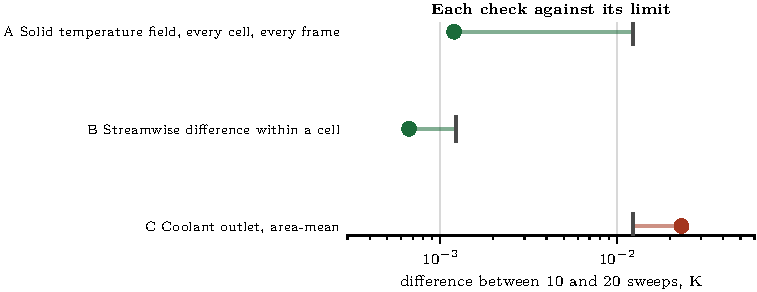
\includegraphics[width=\linewidth]{figures_actC_gate/actC_gate_checks.pdf}\\[0.6mm]
{\scriptsize\color{rulegrey}A 0.00120\,/\,0.01234\,K $\cdot$
B 0.00067\,/\,0.00123\,K $\cdot$ C 0.02315\,/\,0.01234\,K}
\end{minipage}

\vspace{1.8mm}
\hrule height 0.3pt
\vspace{1.6mm}

% ===================== THE RUN AND THE GATE ================================
\begin{minipage}[t]{0.475\textwidth}
\hdr{Both arms run clean}
{\footnotesize
\begin{tabular}{@{}p{0.60\linewidth}p{0.34\linewidth}@{}}
\toprule
Steps completed & 1{,}800 of 1{,}800\\
Exit status & 0, both arms\\
Fatal errors & none\\
Final time reached & 900\,s\\
Fields written, both regions & complete\\
Every field newer than the run's own start mark & yes, by 16\,s or more\\
\bottomrule
\end{tabular}}\\[1.0mm]
{\footnotesize
\bl{Ceiling used: 21.0\,\% of 34\,min, 17.3\,\% of 73\,min}
\bl{Stops early: 0. Cap stops: 0}
}\vspace{1.2mm}

\hdr{The gate answers}
{\footnotesize
\begin{tabular}{@{}p{0.40\linewidth}rrl@{}}
\toprule
Difference, 10 v.\ 20 sweeps & measured & limit & \\
\midrule
Solid field, every cell & 0.0012 & 0.0123 & \PASS\\
Streamwise step in a cell & 0.00067 & 0.00123 & \PASS\\
Coolant outlet & 0.0232 & 0.0123 & \FAIL\\
\bottomrule
\end{tabular}}\\[0.8mm]
{\footnotesize All values in K. All three checks are required.}
\end{minipage}
\hfill
\begin{minipage}[t]{0.495\textwidth}
\vspace{-1mm}
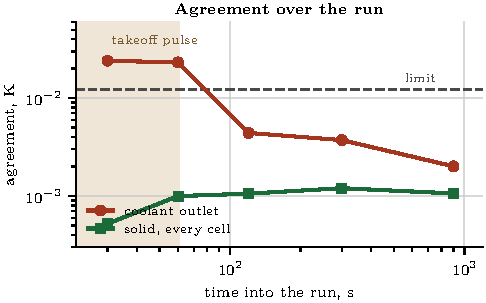
\includegraphics[width=\linewidth]{figures_actC_gate/actC_gate_over_run.pdf}\\[0.6mm]
{\scriptsize\color{rulegrey}Outlet, K: 30\,s 0.02404 $\cdot$ 60\,s 0.02315
$\cdot$ 120\,s 0.00440 $\cdot$ 300\,s 0.00372 $\cdot$ 900\,s 0.00201.
Limit 0.01234\,K}
\end{minipage}

\vspace{1.8mm}
\hrule height 0.3pt
\vspace{1.6mm}

% ===================== THE REFUSAL =========================================
\colorbox{keyfill}{\begin{minipage}{0.985\textwidth}
\vspace{0.8mm}
{\footnotesize\bfseries The gate refuses. Nothing thermal is published.}\\[0.8mm]
{\footnotesize
\bl{Outlet moves 0.02315\,K against a 0.01234\,K limit: $1.88\times$ over}
\bl{0.01234\,K is the smallest difference this case calls a signal}
\bl{A result at that scale sits inside its own numerical spread}
}\vspace{0.4mm}
{\footnotesize\bfseries Withheld:} {\footnotesize cell temperatures; the
temperature rise; the coolant outlet temperature; the three acceptance
criteria; the energy ledger. The reader controls are never reached: the gate is
evaluated first.}
\vspace{0.9mm}
\end{minipage}}

\vspace{1.8mm}

% ===================== WHAT IS SOLID, AND WHAT IS NEXT =====================
\begin{minipage}[t]{0.30\textwidth}
\vspace{-1mm}
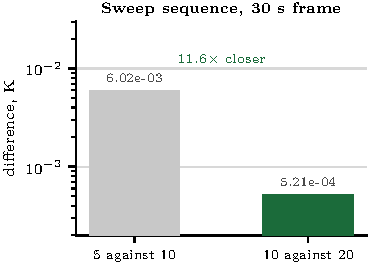
\includegraphics[width=\linewidth]{figures_actC_gate/actC_gate_sequence.pdf}\\[0.6mm]
{\scriptsize\color{rulegrey}5$\to$10: 0.00602\,K $\cdot$ 10$\to$20:
0.00052\,K $\cdot$ ratio $11.6\times$}
\end{minipage}
\hfill
\begin{minipage}[t]{0.325\textwidth}
\hdr{What is solid}
{\footnotesize
\bl{30\,s frame: 5$\to$10 gives 0.00602\,K}
\bl{10$\to$20 gives 0.00052\,K: $11.6\times$ closer}
\bl{Solid converging, coolant not}
\bl{Both measured; one verdict cannot separate them}
}
\end{minipage}
\hfill
\begin{minipage}[t]{0.325\textwidth}
\hdr{Cost}
{\footnotesize
\begin{tabular}{@{}p{0.40\linewidth}rr@{}}
\toprule
 & planned & actual\\
\midrule
Arm 1, 10 sweeps & 8.3 min & 7.2 min\\
Arm 2, 20 sweeps & 18.1 min & 12.6 min\\
Total & 26.4 min & 19.8 min\\
Spend & \$0.022 & \$0.017\\
\bottomrule
\end{tabular}}\\[0.7mm]
{\footnotesize
\bl{Predicted 26.39, used 19.763\,min}
\bl{\textbf{25.1\,\% UNDER prediction}}
\bl{Sweep doubling costs $1.77\times$, planned $2.18\times$}
\bl{Ceiling 390\,min, 5.1\,\% used}
}
\end{minipage}

\vspace{2.0mm}
\hrule height 0.3pt
\vspace{1.4mm}

\hdr{The priced next step}
{\footnotesize
\begin{tabular}{@{}p{0.30\linewidth}p{0.44\linewidth}p{0.20\linewidth}@{}}
\toprule
Lever & Why & Cost\\
\midrule
Finer time step through the pulse & Addresses the cause: air crosses a channel
in 31\,ms, Courant near 1600, load stepping & to be priced\\
More outer sweeps & Weaker: 40 sweeps lands near the 0.01234\,K limit and
leaves the cause alone & about 22 min\\
\bottomrule
\end{tabular}}\\[1.0mm]

{\footnotesize\bfseries The honest sentence: the run completes, the gate
refuses it, and no thermal result exists.}

\end{document}
